\section{Eingangskennlinie}
\subsection{Experimentelle Durchf\"uhrung}
Zu\"achst wir die Schaltung wie in der Abbildung 1 auf dem Steckbrett aufgebaut. In diesem Versuch wird die Eingangskennlinie \textbf{I$_B$ $=$ f(U$_{BE}$)} des NPN-Transistors BC~547C aufgenommen. Aus dieser Kennlinie wird auschli\ss end der Gro\ss signalwiderstand R$_{BE}$ sowie der Kleinsignalwiderstand r$_{BE}$ f\"ur verschiedene Arbeitspunkte ermittelt. \\
\begin{figure}[!h]
\begin{center}
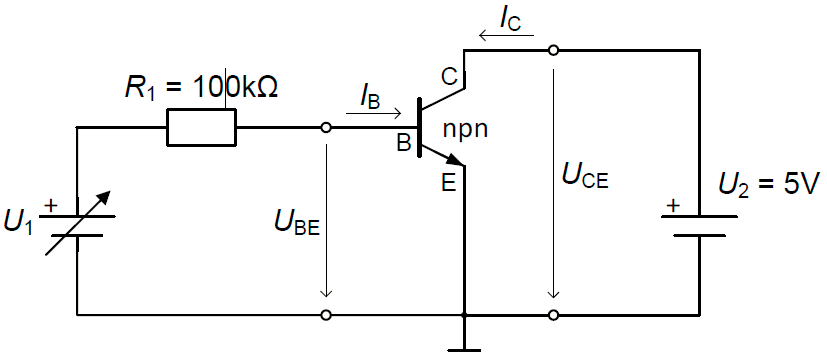
\includegraphics[width=0.9\textwidth]{eingangsKennlinie}
\caption{Der Versuchsaufbau zur Bestimmung der Eingangskennlinie des Transistors}\label{fig:versuch1}
\end{center}
\end{figure}

\subsection{Ergebnisse und Diskussion}
In Tabelle 1 befinden sich die Ergebnisse der Messung und der Simulation f\"ur die Spannung U$_{BE}$ in Abh\"angigkeit von dem Basisstrom I$_B$B.
\begin{figure}[!h]
\begin{center}
\textbf{Tabelle 1: Aufgenommene Messwerte von U$_{BE}$ in Abh\"angigkeit von I$_B$ f\"ur U$_2$ $=$ 5~$V$ } \\[0.2cm]
%\caption{ }
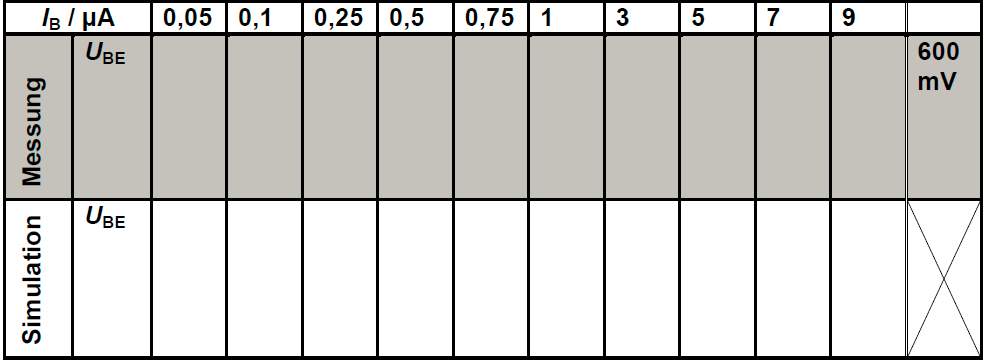
\includegraphics[width=0.8\textwidth]{ergebnissVersuch1}
\end{center}
\end{figure}
\begin{figure}[!h]
\begin{center}
\vspace{10cm}
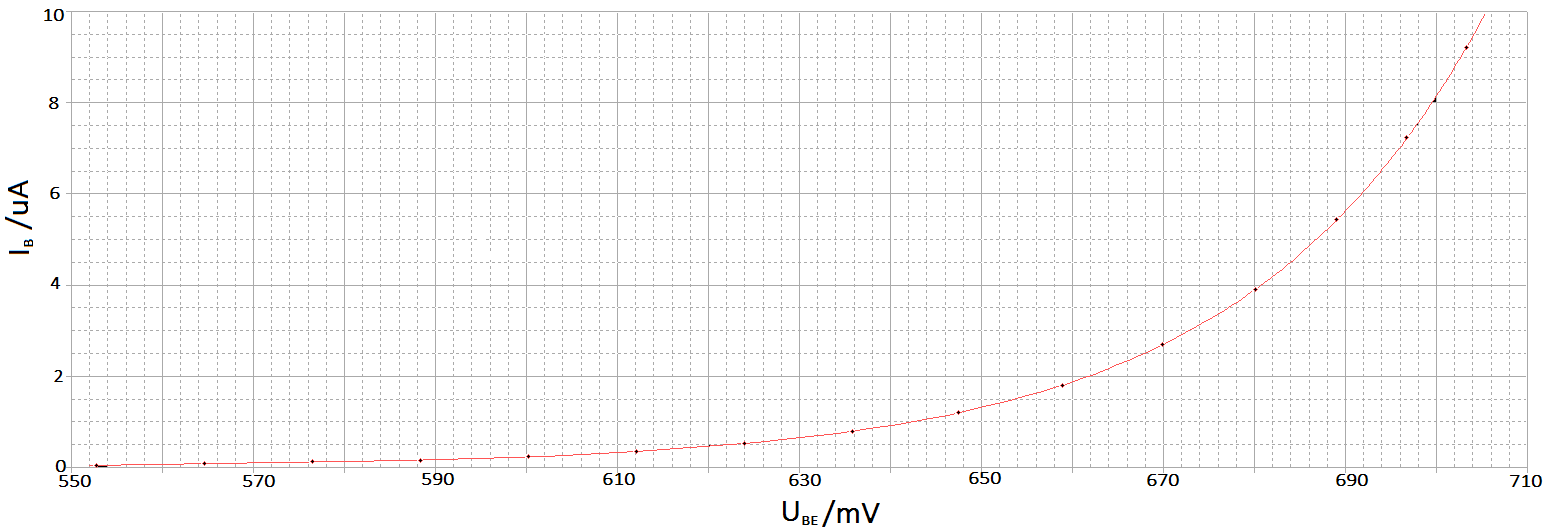
\includegraphics[width=1\textwidth]{Verscuh1}
\caption{Graphische Darstellung der simulierten Ergebnisse}
\end{center}
Abbildung (2) zeigt den Verlauf des Basisstrom in Abh\"angigkeit der Basisemitterspannung. Es zeigt sich, dass der Basisstrom mit dem Verlauf einer \"ublichen Diodenkennlinie \"ubereinstimmt. 
\end{figure}
\begin{equation}
\textbf{R$_{RE}$} = \frac{\textbf{U$_{BE}$}}{\textbf{I$_B$}}
\end{equation}
\begin{equation}
\textbf{r$_{RE}$} = \frac{\textbf{$\Delta$U$_{BE}$}}{\textbf{$\Delta$I$_B$}}
\end{equation}
In der Gleichung (1) bzw. (2) kann der Gro\ss - bzw. Kleinsignalwiderstand bestimmt werden.
\begin{table}[!h]
Um den Gro\ss signalwiderstand bestimmen zu k\"onnen, muss die Spannung U$_{BE}$ \"uber alle drei Arbeitspunkte bestimmt werden:  I$_{B_{\textbf{i}_{\{1,2,3\}}}}$. 
\begin{center}
\begin{tabular}{|l|l|l|}
\hline
Messreihe & U$_{{BE}_{\textbf{Simulation}}}$/$mV$ & U$_{{BE}_{\textbf{Messung}}}$/$mV$\\
\hline
I$_{B_1}$ & 574 & 588 \\
\hline
I$_{B_2}$ & 673 & 672 \\
\hline
I$_{B_3}$ & 659 & 688 \\
\hline
\end{tabular}
\end{center}
\begin{center}
\begin{tabular}{|l|l|l|l|l|l|l|}
\hline
& R$_{BE_{simulation}}$ & R$_{BE_{Messung}}$ \\
\hline
I$_{B_1}$ &  & \\
\hline
I$_{B_2}$ & & \\
\hline
I$_{B_3}$ & & \\
\hline
\end{tabular}
\end{center}
\end{table}
\begin{table}[!h]
\begin{center}
\begin{tabular}{|l|l|l|l|l|l|l|}
\hline
& r$_{BE_{simulation}}$ & r$_{BE_{Messung}}$ \\
\hline
I$_{B_1}$ &  & \\
\hline
I$_{B_2}$ & & \\
\hline
I$_{B_3}$ & & \\
\hline
\end{tabular}
\end{center}
Wegen des nicht linearen Kurvenverlauf ist der Eingangswiderstand r$_{RB}$ bei unterschiedlichen Kennlinienpunkten nicht gleich, da je gr\"o\ss er der Basisstrom ist, desto gr\"o\ss er wird der Widerstand \\
F\"ur den Kleinsignalwiderstand gilt folgende Formal: \begin{equation*}
\textbf{r$_{BE}$} = \frac{U_{Temp}}{I_B}, \textbf{\ \ I$_B$ am Arbeitspunkt}
\end{equation*}
\end{table}
\newpage